\documentclass[12pt,a4paper]{article}

\usepackage[a4paper, top = 2cm, bottom = 2cm, left = 1.5cm, right = 1.5cm]{geometry}
\usepackage[dvipsnames]{xcolor} % Colors

\usepackage{standalone}

\usepackage{setspace}
\usepackage{graphicx}
\usepackage{amsfonts}
\usepackage{amsmath}
\usepackage{tikz}
\usepackage{pdfpages}
\usepackage{epigraph}
\usepackage{csquotes}
\usepackage{natbib}
% Bibliography
\usepackage{xcolor}
\usepackage{hyperref}
\hypersetup{
colorlinks=true,
citecolor=MidnightBlue,
linkcolor=MidnightBlue,
pdfpagemode=FullScreen}

\usepackage{natbib}
\usepackage[noabbrev]{cleveref}
\setcitestyle{authoryear,open={(},close={)}}
\bibliographystyle{plainnat}

\usepackage{subfiles}

\setlength\parindent{0pt}
\spacing{1.2}

\begin{document}

\begin{center}
       \vspace*{4cm}
       \huge\textbf{Project 4} \\
       \vspace{0.4cm}
       \large \textbf{Public Finance in Macroeconomics} \\
       \vspace{0.5cm}
        \large Handed in by the \textcolor{orange}{\textbf{Heterogeneous Geeks}} \\
        \vspace{0.3cm}
        a.k.a. Vivien Voigt, Thong Nguyen, 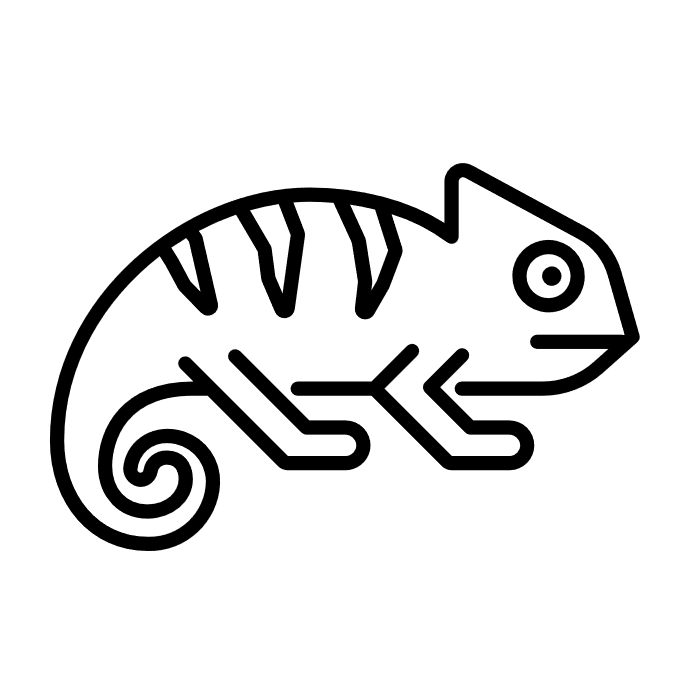
\includegraphics[scale=0.06]{stata_output/geek.png}\\Davide Difino \& Celina Proffen \\
       \vspace{1.5cm}
       \vfill



        Project in the context of Prof. Ludwig's course: \\
        \textbf{Public Finance in Macroeconomics: Heterogenous Agent Models}\\
        at the Graduate School of Economics, Finance, and Management
       \vspace{0.8cm}
   \end{center}

\newpage

%%%%%%%%%%%%%%%%%%%%%%%%%%%%%%%%%%%%%%%%%%%%%%%%%%%%%%%%%%%%%%%%%%%%
%%%%%%%%%%%%%%%%%%%%%%%%%%%%%%%%%%%%%%%%%%%%%%%%%%%%%%%%%%%%%%%%%%%%

\section*{Problem 1: Smoothed Income Profiles over the Life Cycle}

\textbf{General Remark:} Please have a look at our commented code. We refer to the measures of income $yhh5$ and $yhh6$ for pre- and post-government income respectively. As required, we deflate these measures and apply logarithms before computing predicted values and residuals. \\

\textbf{Interpretation income profiles:} For both, married and single household heads, the pre-government income varies more greatly over the entire life-cycle than the post government income does (note the y-axis on the graphs below). This can be explained by the pension payments paid to older individuals that prevent a drastic fall in income after retirement. \\ Furthermore, it is to note that married household heads tend to be associated with higher household incomes albeit a similar pattern than single ones. The reason for this is likely to be that the household combines the incomes of multiple (potentially working) persons that are part of the household when a household head is married. However, incomes do not become twice the size\footnote{This is true even after keeping in mind that we are working on a log scale.} as one could have expected. This could be due to various reasons. E.g. it could be that one partner stays home for childcare, only works partially or that lower-earning people are more likely to be married. This is supported by figures 3 and 4 showing that the annual hours worked of single households are differently distributed than of married households. \\

\begin{figure}[h]
  \centering
  \begin{minipage}[b]{0.45\textwidth}
    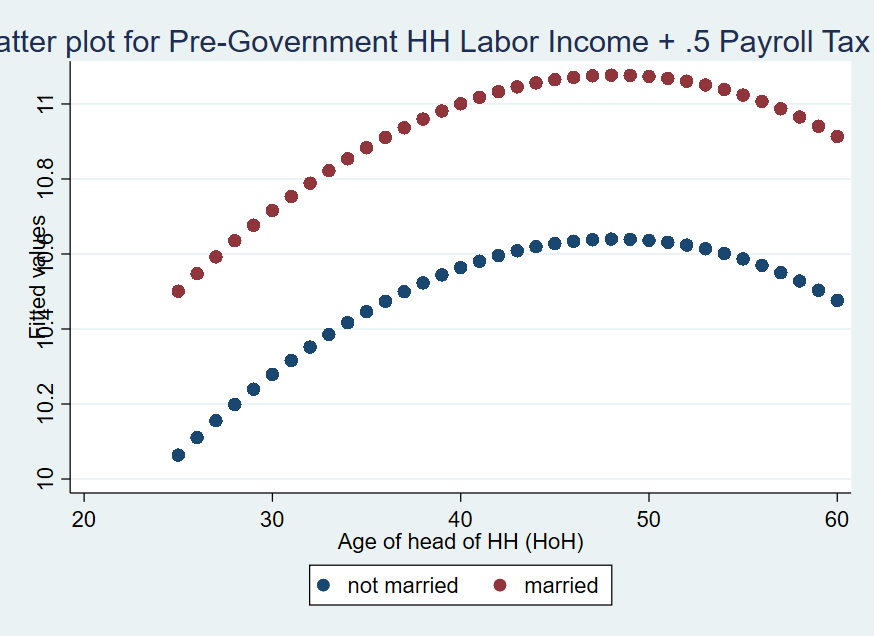
\includegraphics[width=\textwidth]{stata_output/smoothed_yy5_hat.png}
    \caption{Based on $YHH5$}
  \end{minipage}
  \hfill
  \begin{minipage}[b]{0.45\textwidth}
    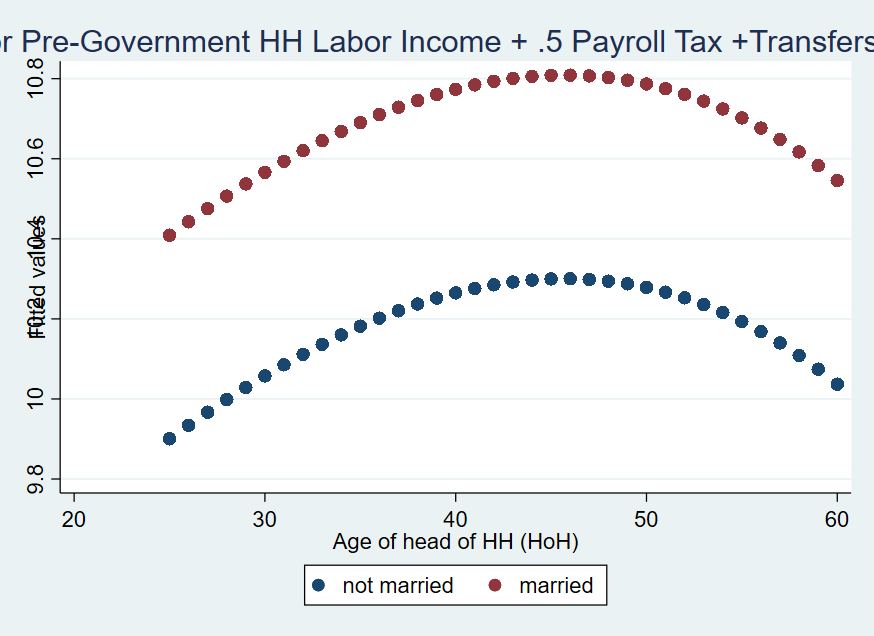
\includegraphics[width=\textwidth]{stata_output/smoothed_yy6_hat.png}
    \caption{Based on $YHH6$}
  \end{minipage}
\end{figure}

\textbf{Interpretation Residual Variances:} The Pre-government residual income variance is $\sigma^2_{\Tilde{y}_{-Pre}} = 0.72517049$ and the equivalent for the post-government income is $\sigma^2_{\Tilde{y}_{-Post}} = 0.60099632$. As can be seen the latter is considerably smaller than the fist, which is in line with the redistributive effect of taxes. 

\newpage

\begin{figure}[h]
  \centering
  \begin{minipage}[b]{0.45\textwidth}
    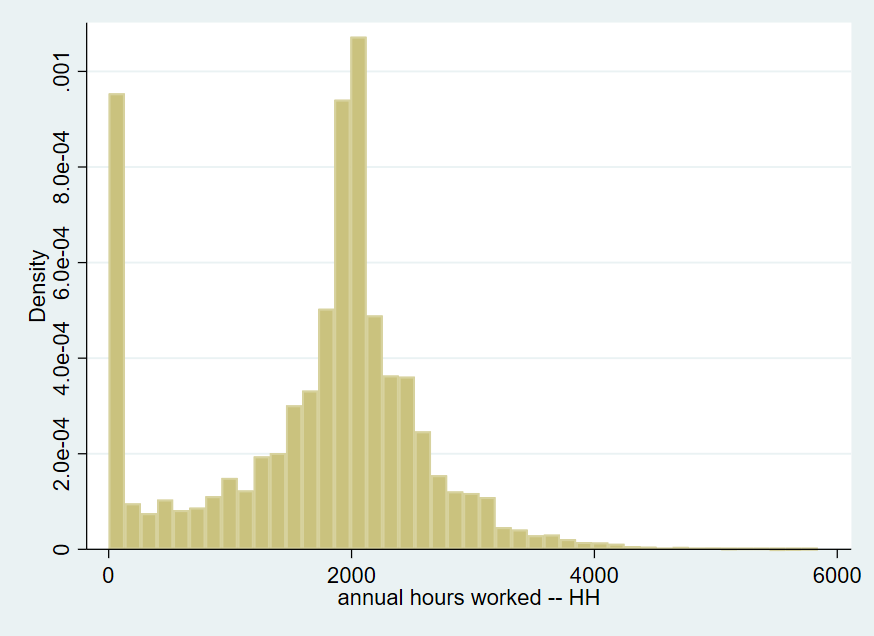
\includegraphics[width=\textwidth]{stata_output/Hrs_hh_nm.png}
    \caption{Single household - annual hours worked}
  \end{minipage}
  \hfill
  \begin{minipage}[b]{0.45\textwidth}
    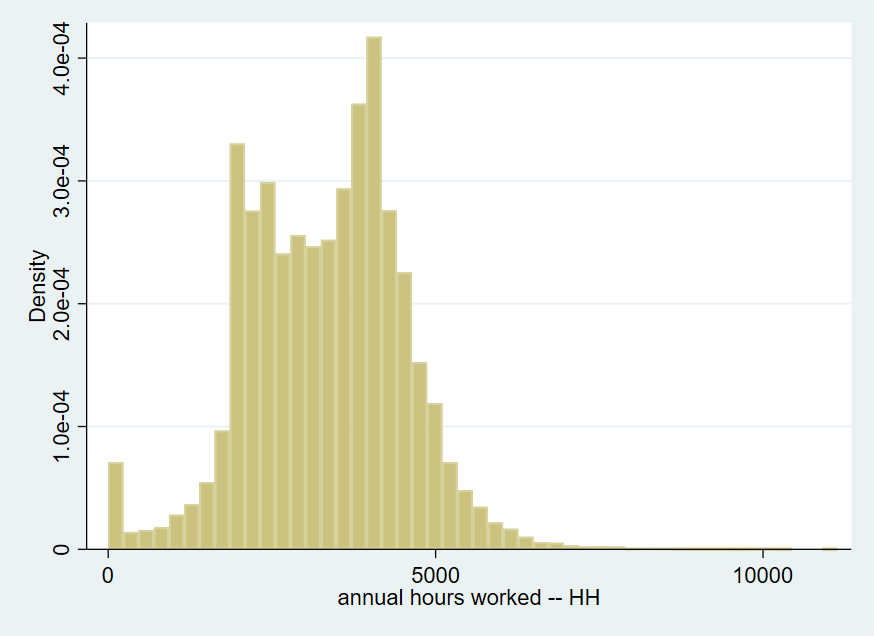
\includegraphics[width=\textwidth]{stata_output/Hrs_hh_m.png}
    \caption{Married household - annual hours worked}
  \end{minipage}
\end{figure}


\section*{Problem 2: Theoretical Income Process}

The following values where retrieved from the data:

\begin{table}[h]
\begin{tabular}{|l|l|l|}
\hline
\textbf{Variable} & \textbf{Pre government income} & \textbf{Post government income}  \\ \hline
$\rho$                        &    0.9088825   (0.0151314)  &  0.9080964   (0.0137734)         \\ \hline
$\sigma^2_z$                  &   16.15252   (69.36648)  &  41.87742   (68.17502)        \\ \hline
$\sigma^2_\nu$                &   0.0861262   (0.0185558)  &   0.0644558   (0.0150432)        \\ \hline
$\sigma^2_\epsilon$           &   0.2144817   (0.0164309)  &   0.1489496   (0.0121499)        \\ \hline
$\sigma^2_{\Tilde{y}}$        &   0.7096516647             &   0.5165103823                   \\ \hline
\end{tabular}
\caption{The estimates for all variables but $\sigma^2_{\Tilde{y}}$ stem from estimations in the stata do.file handed in together with this project. The estimate of $\sigma^2_{\Tilde{y}}$ is computed using the formula given in the project instructions and also derived below.}
\end{table}

Remember from the project instructions the following two equations:
\begin{equation}\tag{1a}
    \Tilde{y}_{ijt} = z_{ijt} - \epsilon_{ijt}
\end{equation}
\begin{equation}\tag{1b}
    z_{ijt} = \rho z_{ij-1t-1} - \nu_{ijt}
\end{equation}

Let's start by deriving a new representation for residual income from (1) in the project instructions. First note that (1a) implies
\begin{align}
    z_{ij-1t-1} = \Tilde{y}_{ij-1t-1} - \epsilon_{ij-1t-1}
\end{align}
As $\epsilon$ is equally distributed over ages and individuals this can be rewritten as:
\begin{align}
    z_{ij-1t-1} = \Tilde{y}_{ij-1t-1} - \epsilon_{t-1}
\end{align}
Inserting the equation above in (1b) and noticing that $\nu$ is also distributed identically over ages and individuals:
\begin{align}
    z_{ijt} & = \rho(\Tilde{y}_{ij-1t-1} - \epsilon_{t-1}) + \nu_{ijt} \\
            & = \rho(\Tilde{y}_{ij-1t-1} - \epsilon_{t-1}) + \nu_{t}
\end{align}
Plugging in this transformation in (1a) yields:
\begin{align}
    \Tilde{y}_{ijt} = \rho\Tilde{y}_{ij-1t-1}  + \nu_{t} + \epsilon_t - \rho \epsilon_{t-1}
\end{align}

Now, for deriving the variance of $\Tilde{y}$, i.e. $\sigma^2_{\Tilde{y}}$, \textbf{a key assumption will be that all shocks are orthogonal to each other}, meaning that their co-variance is equal to zero. Also, it is important to assume that the process is weakly stationary (i.e. (co)variances do not change over time). 

Taking the variance of the equation above yields:
\begin{align}
    \sigma^2_{\Tilde{y}} & = \rho^2 \sigma^2_{\Tilde{y}} + \sigma^2_\nu + (1-\rho^2)\sigma^2_\epsilon \\
                         & = \frac{\sigma^2_\nu}{(1-\rho^2)} + \sigma^2_\epsilon
\end{align}
This proves the statement. The formula was used to estimate the variance of the residual income $\sigma^2_{\Tilde{y}}$.
\end{document}
